
\documentclass[11pt,paper=a4,answers]{exam}

\newcommand*{\renameenviron}[1]{%
	\expandafter\let\csname exam-#1\expandafter\endcsname
	\csname #1\endcsname
	\expandafter\let\csname endexam-#1\expandafter\endcsname
	\csname end#1\endcsname
	\expandafter\let\csname #1\endcsname\relax
	\expandafter\let\csname end#1\endcsname\relax
}
\renameenviron{framed}
\renameenviron{shaded}
\renameenviron{leftbar}
\usepackage{framed}

\usepackage[utf8]{inputenc}		% Codificacao do documento (conversão automática dos acentos)
\usepackage{graphicx,lastpage}
\usepackage{epstopdf}
\usepackage{upgreek}
\usepackage{censor}
%\usepackage{framed}
\usepackage[brazilian,hyperpageref]{backref}	 % Paginas com as citações na bibl
\usepackage[brazilian]{babel}



\censorruledepth=-.2ex
\censorruleheight=.1ex
\hyphenpenalty 10000
\usepackage[paperheight=10.5in,paperwidth=8.27in,bindingoffset=0in,left=0.8in,right=1in,
top=0.7in,bottom=1in,headsep=.5\baselineskip]{geometry}


\flushbottom
\usepackage[normalem]{ulem}
\renewcommand\ULthickness{2pt}   %%---> For changing thickness of underline
\setlength\ULdepth{1.5ex}%\maxdimen ---> For changing depth of underline
\renewcommand{\baselinestretch}{1}
\pagestyle{empty}

\pagestyle{headandfoot}
\headrule
\newcommand{\continuedmessage}{%
	\ifcontinuation{\footnotesize Question \ContinuedQuestion\ continues\ldots}{}%
}
\runningheader{\footnotesize EEL7278 -- Eletrônica Industrial}
{\footnotesize }
{\footnotesize P\'agina \thepage\ de \numpages}
\footrule
\footer{\footnotesize Lista de Exercícios 06 -- \today}
{}
{\ifincomplete{\footnotesize Pergunta  \IncompleteQuestion\ continua na pr\'oxima p\'agina \ldots}{\iflastpage{\footnotesize Fim do exercício!}{\footnotesize Continua na pr\'oxima p\'agina\ldots}}}

\usepackage{cleveref}
\crefname{figure}{figure}{figures}
\crefname{question}{question}{questions}


%==============================================================
\begin{document}
	
	%% \thispagestyle{empty}	
	\noindent
	\begin{minipage}[l]{.1\textwidth}%
		\noindent
		
\includegraphics[width=2\textwidth]{logo-ufsc}
	\end{minipage}
	\hfill
	\begin{minipage}[r]{.8\textwidth}%
		\begin{center}
			{\large \bfseries UNIVERSIDADE FEDERAL DE SANTA CATARINA \par
				\large Departamento de Engenharia Elétrica e Eletrônica \\[4pt]
			%	\vspace{0.5cm}
				Eletrônica Industrial {(EEL7278)}  \par
				\vspace{0.5cm}
				\huge Lista de Exercícios 06
				}
			%  \vspace{0.5cm}
		\end{center}
	\end{minipage}	
		
		\par
		\noindent
		\uline
%		\uline{Tempo: 90 min.   \hfill \normalsize\emph{\underline{Term}} \hfill  }
	\hfill 	
			
\par
\bigskip\bigskip
\begin{minipage}[t]{.6\textwidth}%
	Professor: Adriano Ruseler \par
	Semestre: 2015/2 \par
	Aluno: \makebox[2.5in]{\hrulefill} \par
	
\end{minipage}%
\hfill
\begin{minipage}[t]{.4\textwidth}%
	Turma:  07202A \par
     \par
	Matricula: \makebox[1.5in]{\hrulefill} \par
\end{minipage}
\par
\bigskip




\begin{framed}
	\centering Lista de exercícios referente a\\ \raggedright
	 \textbf{Aula 06 -- Retificador Trifásico de Onda Completa a Tiristor }
\end{framed}


		
\begin{questions}
			
\pointsinrightmargin
\pointsdroppedatright
\marksnotpoints
%\marginpointname{mark}
\pointpoints{mark}{marks}
\pointformat{\boldmath\themarginpoints}
\bracketedpoints
			
			
			\question[05]
			\label{Q:revisao}
			
		Monte no simulador PSIM a estrutura apresentada em aula, utilizando o bloco contendo a ponte retificadora trifásica.
						\begin{enumerate}
							\item Verifique que para $\alpha = 0$ a ponte a tiristor se comporta como caso particular da ponte a diodos.
							\item Obtenha a tensão na resistência de carga.
							\item Calcule os valores eficazes e médios das correntes nos tiristores para $\alpha=60$.
						\end{enumerate}
						
		\begin{figure}[!h]
\centering
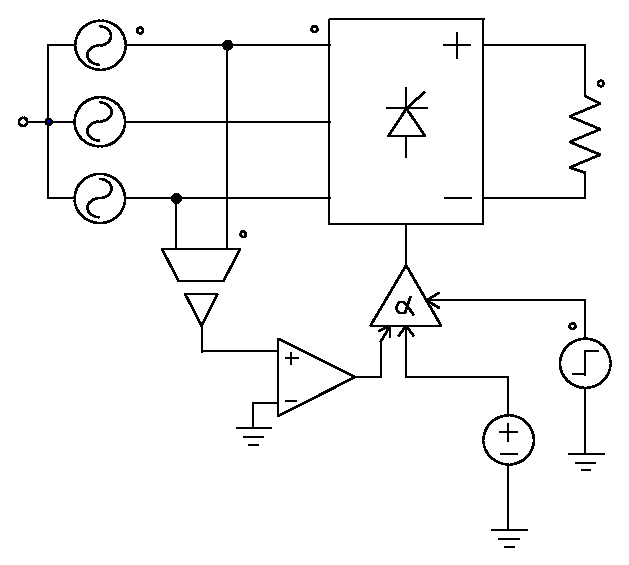
\includegraphics[width=0.5\linewidth]{figuras/SimularEstruturaBloco}
\caption{Estrutura simulada em Aula.}
\label{fig:SimularEstruturaBloco}
\end{figure}
		
			\droppoints
		
		
		
		
		
			
			\question[06]
			\label{Q:perunit}
Implemente o exercício \ref{Q:revisao} utilizando componentes discretos conforme a figura \ref{fig:TiristorDiscreto}.

\begin{figure}[!h]
\centering
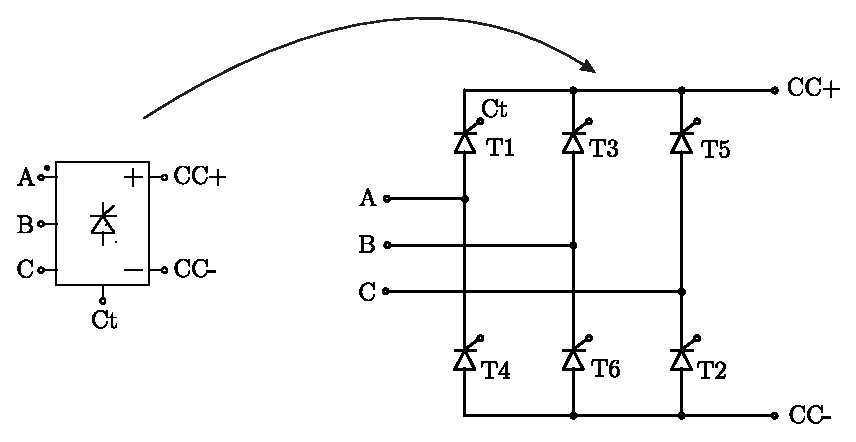
\includegraphics[width=0.7\linewidth]{figuras/TiristorDiscreto}
\caption{Implemente a versão discreta do retificador trifásico a tiristor.}
\label{fig:TiristorDiscreto}
\end{figure}

			\droppoints
			
						
			\question[07]
			\label{Q:ExPSIM}
			
			
	\begin{figure}[!h]
\centering
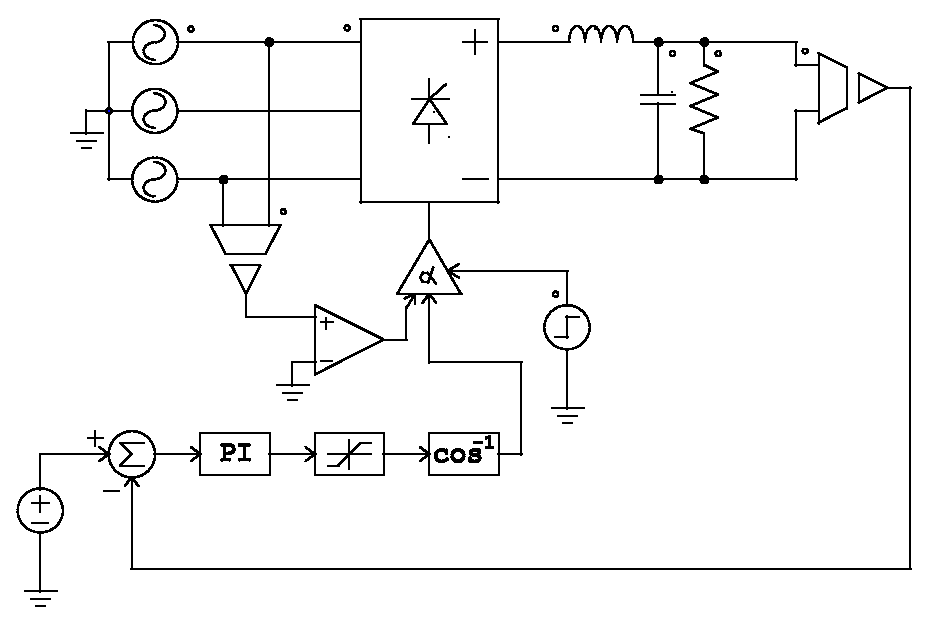
\includegraphics[width=0.7\linewidth]{figuras/ExPSIM}
\caption{Exemplo do controle de uma ponte retificadora a tiristores.}
\label{fig:ExPSIM}
\end{figure}
		
O software de simulação PSIM possui uma pasta com exemplos em seu diretório de instalação. Procure o exemplo apresentado na figura \ref{fig:ExPSIM}	e faça uma simulação exploratória.		
			
			
\droppoints
			
			
			
			
			
			
			
			\question[8]
			\label{Q:Desafio}
	Monte no simulador PSIM a estrutura pentafásica apresentada na figura com carga resistiva.
	\begin{enumerate}
		\item Verifique que para $\alpha = 0$ a ponte a tiristor se comporta como caso particular da ponte a diodos.
		\item Obtenha a tensão na resistência de carga.
		\item Calcule os valores eficazes e médios das correntes nos tiristores para $\alpha=45$.
	\end{enumerate}
	
	\begin{figure}[!h]
		\centering
		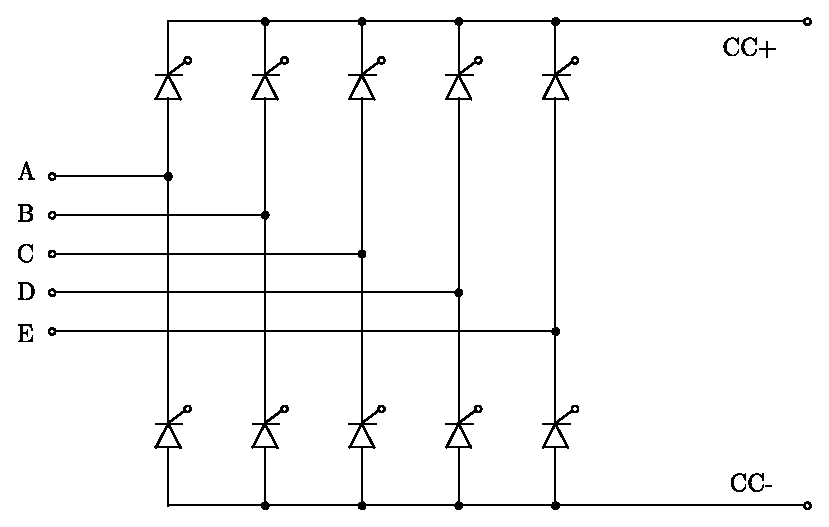
\includegraphics[width=0.7\linewidth]{figuras/TiristorPentafase}
		\caption{Estrutura pentafásica proposta como desafio.}
		\label{fig:TiristorPentafase}
	\end{figure}
			

			
			
		
			
	
			
			

		\end{questions}
		\begin{center}
			\rule{.5\textwidth}{1pt}
		\end{center}
	\end{document} 